


\chapter{Spatial Capture-Recapture for Unmarked Populations}
\markboth{Chapter 14 }{}
\label{chapt.scr-unmarked}

\vspace{0.3cm}


Traditional capture-recapture models share the fundamental
assumption that each individual in a population can be uniquely
identified when captured. This can often be accomplished
by marking individuals with color bands, ear tags, or some other
artifical mark that can be read in the field. For other species, such as
tigers or marbled salamanders, individuals can be easily identified
using only their natural markings. In a great number of cases, however,
species do not possess sufficient natural markings and are too
difficult to capture to make it practical to apply artifical marks. So
we must throw up our hands and not study these species. End of
chapter.

When capture-recapture methods are not a viable option, researchers
often collect simple count data or even detection/non-detection data
to estimate population parameters. These data are often analyzed using
Poisson regression or logistic regression, perhaps with random
effects; but when detection is imperfect, as it almost always is,
these methods cannot be used to obtain unbiased estimates of
population size or occurrence probability. Even when these data are
used an index of abundance or occurrence, standard models may yield
unreliable results when covariates affect both the state variable and
detection probability. A classic example is the finding by
\citet{bibby_buckland:1987} who reported that the probability of detecting
songbirds in restocked confier plantations decreased with vegetation
height; whereas population density was positively related to
vegetation height. This intuitive and common phenomenon has led to the
development a vast number of methods to model population size or
density while controlling for factors affecting detection
probability. A review of these models is beyond the scope of this
chapter, but we mention a few deficiencies of existing methods
that warrant the exploration of alternatives.

Distance sampling, which we briefly introduced in chapter XXXX,
is perhaps the most widely used method for
estimating population density when individuals are unmarked and
detection probability is less than one. This class of methods is known
to work impecibly when estimating the number of stakes in a field or
the number of duck nests in a wetland. It can also work very well in
more interesting situations; however, %In many other situations,
common issues such as animal movement and measurement error may result in
substantial bias. In addition, traditional distance sampling methods
assume that individuals are randomly located with respect to the
observer and are available for detection (but see
\citet{johnson_etal:2010,chandler_etal:2011}). % Add ISSJ paper too
Most other
methods, such as double-observer sampling and repeated counts, can be
used to estimate population size, but as with traditional CR methods,
it may be difficult to covert abundance estimates to
density estimates because the effective area sampled is unknown. We
mention these issues not to suggest that existing models do not have
value---
indeed we believe that they can be used to obtain reliable density
estimates in many situations---rather our aim to highlight the need for
alternative methods when the assumptions of existing methods cannot be
met. Additionally, the model we develop in this chapter serves as the
foundation for a broad class of SCR models in which all or some of the
individuals cannot be uniquely identified.

In this chapter we highlight the work of \citet{chandler_royle:2012}
who demonstrated that the individual recognition assumption of
CR models is not a requirement of spatial capture-recapture
models. The ability to fit
SCR models to data from unmarked populations has important
consequences in several respects. For one, it means that SCR models can
be applied to data collected using methods like points counts in which
observers record simple counts of animals at an array of survey
points. This development also has important implications for
traditional SCR studies because many resulting datasets include some
individuals that cannnot be identified due to poor photo quality or
the indistiguishable natural markings.


In order to apply SCR models to data collected unmarked animals, one
requirement is critial---counts must be spatially correlated. Of
course, this condition holds true in virtually all SCR models since
animals are often detected at more than one trap. In fact, efficient
SCR designs should try to ensure correlation in counts among
neighboring traps because this is the primary source of information
about the encounter rate parameter, $\sigma$.

%Although ``unmarked SCR'' models represent an important development,
%we will see that they are not without their limitations. For example,
%when all individuals are unmarked, we can expect extreme sensitivity
%to the priors as well as skewed posterior distributions in typical
%sample sizes. Nonetheless,






\section{Data Requirements and Survey Designs}





\section{Encounter Histories as Latent Variables}

Just when you thought we ran out of things to treat as latent
variables, we are now going to regard even the data itself as latent.


State model is the same as other SCR models.


It is natural to regard the encounter rate of an individual
as a function of the Euclidean distance between the individual's
activity center and the trap location, $d_{ir} = \| {\bf x_r} - {\bf
  s_i} \|$.
To be precise about this, we let $z_{irt}$ be the encounter frequency
of
individual $i$ in trap $r$ during occasion $t$. While we will adopt the view
that  the variables $z_{irt}$ are latent variables (see below), it will
be convenient to formulate the model in terms of these variables.

Therefore, we assume that the expected encounter frequency of an
individual in some trap is related to $d_{ir}$ as follows:
\[
E[z_{irt}] = \lambda_{ir} = \lambda_0 k_{ir}
\]
where $\lambda_0$ is the expected encounter rate at $d=0$ and $k_{ir}$
is some positive-valued
function of distance $d_{ir}$. We assume
\[
k_{ir} = exp(-d_{ir}^2 / 2\sigma^2)
\]
where $\sigma$ is a scale parameter related to home
range size. $\sigma$ also determines the degree of correlation among
counts since animals with large home ranges are more likely to be
detected at multiple traps relative animals with small home ranges.
The phenomenon is analogous to correlation induced by averaging
spatial noise, in which case there is a unique correlation between the
smoothing kernel and the induced covariance function
\citep{higdon:02}.

We emphasize that our focus is on
situations in which individuals are {\it not}
uniquely identifiable, and therefore the encounter frequencies
for each individual
cannot be observed, and so they are latent variables. We assume that
these latent variables are realizations from a Poisson distribution
with mean $\lambda_{ir}$:
\begin{equation}
 z_{irt} \sim \mbox{Poisson}(\lambda_{ir}).
\label{eq.latentPoisson}
\end{equation}
In traditional SCR models, $z_{irt}$ are the observed data, {\it
  i.e.}, the frequency of encounters of individual $i$ at trap $r$ on
replicate survey $t$. However, when individual identity is not known,
the observed data are the sample- and trap-specific totals,
aggregated over all individuals:
\[
n_{rt} = \sum_{i=1}^{N} z_{irt}.
\]
Thus the data required by our model are a reduced-information
summary of the latent encounter histories.


Under the Poisson encounter model we have that
\begin{equation}
n_{rt} \sim \mbox{Poisson}( \Lambda_{r} )
\label{eq:nagg}
\end{equation}
where
\[
 \Lambda_{r} = \lambda_{0} \sum_{i} k_{ir}.
\]
Further, because $\Lambda_{r}$ does not depend on $t$, we can
aggregate the replicated counts, defining
$n_{r.} = \sum_{t} n_{rt}$ and then
\[
 n_{r.} \sim \mbox{Poisson}( T \Lambda_{r} )
\]
As such, $T$ and $\lambda_{0}$ serve equivalent roles as affecting
baseline encounter rate.
This formulation of the model in terms of the aggregate count
simplifies computations as the latent variables
$z_{irt}$ do not need to be updated in the MCMC estimation
scheme (see below). However, retaining $z_{irt}$
in the formulation of the model
is important if some individuals are uniquely marked, in which case
modifying
the MCMC algorithm (see below) to include both types of data is
trivial. This is because uniquely identifiable individuals produce
observations of some of the $z_{irt}$ variables.

We imagine that other observation models
might be possible (see Discussion) although we focus here on the
Poisson encounter model because it has considerable relevance to
animal surveys, and has additional methodological context related to
point process models which we address in the Discussion.





\section{Estimation by MCMC}
\label{s:mcmc}

We adopt a Bayesian framework for inference allowing estimation of $N$
while retaining the formulation of the model that is conditional on
the latent activity centers $\bf s_i$.
Specifically, we employ Markov chain Monte Carlo
(MCMC) to simulate posterior distributions of the parameters. However,
the fact that $N$ is unknown presents a
technical challenge because the size of the parameter space can change
with each MC iteration. To resolve this, we
adopt the formulation of data augmentation in \citet{royleEA07_DA} who
used a specific prior construction for $N$ in terms of individual level
Bernoulli trials. In particular, we assume $N \sim \mbox{Unif}(0,M)$
for some large integer $M$. We construct this prior by assuming
$N|M,\phi \sim \mbox{Bin}(M,\phi)$ and $\phi \sim \mbox{DUnif}(0,1)$
which implies, marginally, that $N$ has the requisite
$\mbox{DUnif}(0,M)$ distribution. However
the hierarchical formulation of the prior suggests an implementation
in which we introduce a set of latent indicator variables $w_{i} \sim
\mbox{Bern}(\phi)$ and, furthermore, the model implies
that $z_{irt}$ are obtained
from the specified distribution (Eq. \ref{eq.latentPoisson})
if $w_{i} = 1$, or if
$w_{i}=0$, %the model implies that
$z_{irt} =0$ with probability 1. In
effect, extending the model in this way induces a reparameterization
for the latent counts %$z_{irt}$
that is a zero-inflated version
of the original conditional-on-$N$ model. Specifically, the model
under
data augmentation becomes
\begin{eqnarray*}
 z_{irt}|w_{i} &\sim & \mbox{Poisson}(\lambda_{ir} w_i) \\
 w_{i} & \sim & \mbox{Bern}(\phi)
\end{eqnarray*}
Under this formulation $N = \sum_{i=1}^{M} w_i$, and population
density is simply $D = N/A({\cal S})$ where $A({\cal S})$ is the area of the
point process state-space ${\cal S}$.

We developed two distinct MCMC implementations for this model (\ref{suppA}). In the
first, we devised an algorithm for the model conditional on the latent
variables $z_{irt}$. This formulation is useful for problems in which
one or more individual identities are available, in which case the
$z_{irt}$ are observable for those individuals. The unobserved
$z_{irt}$ are easily updated using their full-conditional
distribution which is multinomial with sample size $n_{rt}$. The
remaining parameters are updated using Metropolis-Hastings steps (see
\ref{suppA}).  In the second formulation of the algorithm we applied
the Metropolis-Hastings algorithm to the model {\it unconditional} on
the $z_{irt}$ variables. In that case, the marginal distribution for
$n_{rt}$ is precisely Eq.~\ref{eq:nagg}.  This algorithm is slightly more
convenient because
it avoids having to update the $z_{irt}$ variables of which there are many.




\section{Northern Parula Example}



To apply our model to data collected in the field, we designed a point
count study of the northern parula ({\it Parula americana}), a
Neotropical-Nearctic migratory passerine. This species defends
well-defined territories during the breeding season
\citep{Moldenhaer_NOPAbna}, and thus our modeling effort was focused
on estimating the number and location of territory centers. Points
were located on a 50-m grid to ensure spatial
correlation. This small grid spacing contrasts with the conventional
practice of spacing points by $>$ 200 m to obtain \emph{i.i.d.}
counts. Figure~\ref{fig:nopaDat} depicts the spatially-correlated
counts ($n_{r.}$) from the 105 point count locations
surveyed three times each during June 2006
at the Patuxent Wildlife Research Center in Laurel Maryland, USA.
A total of 226 detections were made with a maximum count of 4 during a
single survey. At 38 points, no warblers were detected. All but one of
the detections were of singing males, and this one observation was
not included in the analysis.


%\begin{comment}

\begin{figure}
  \centering
  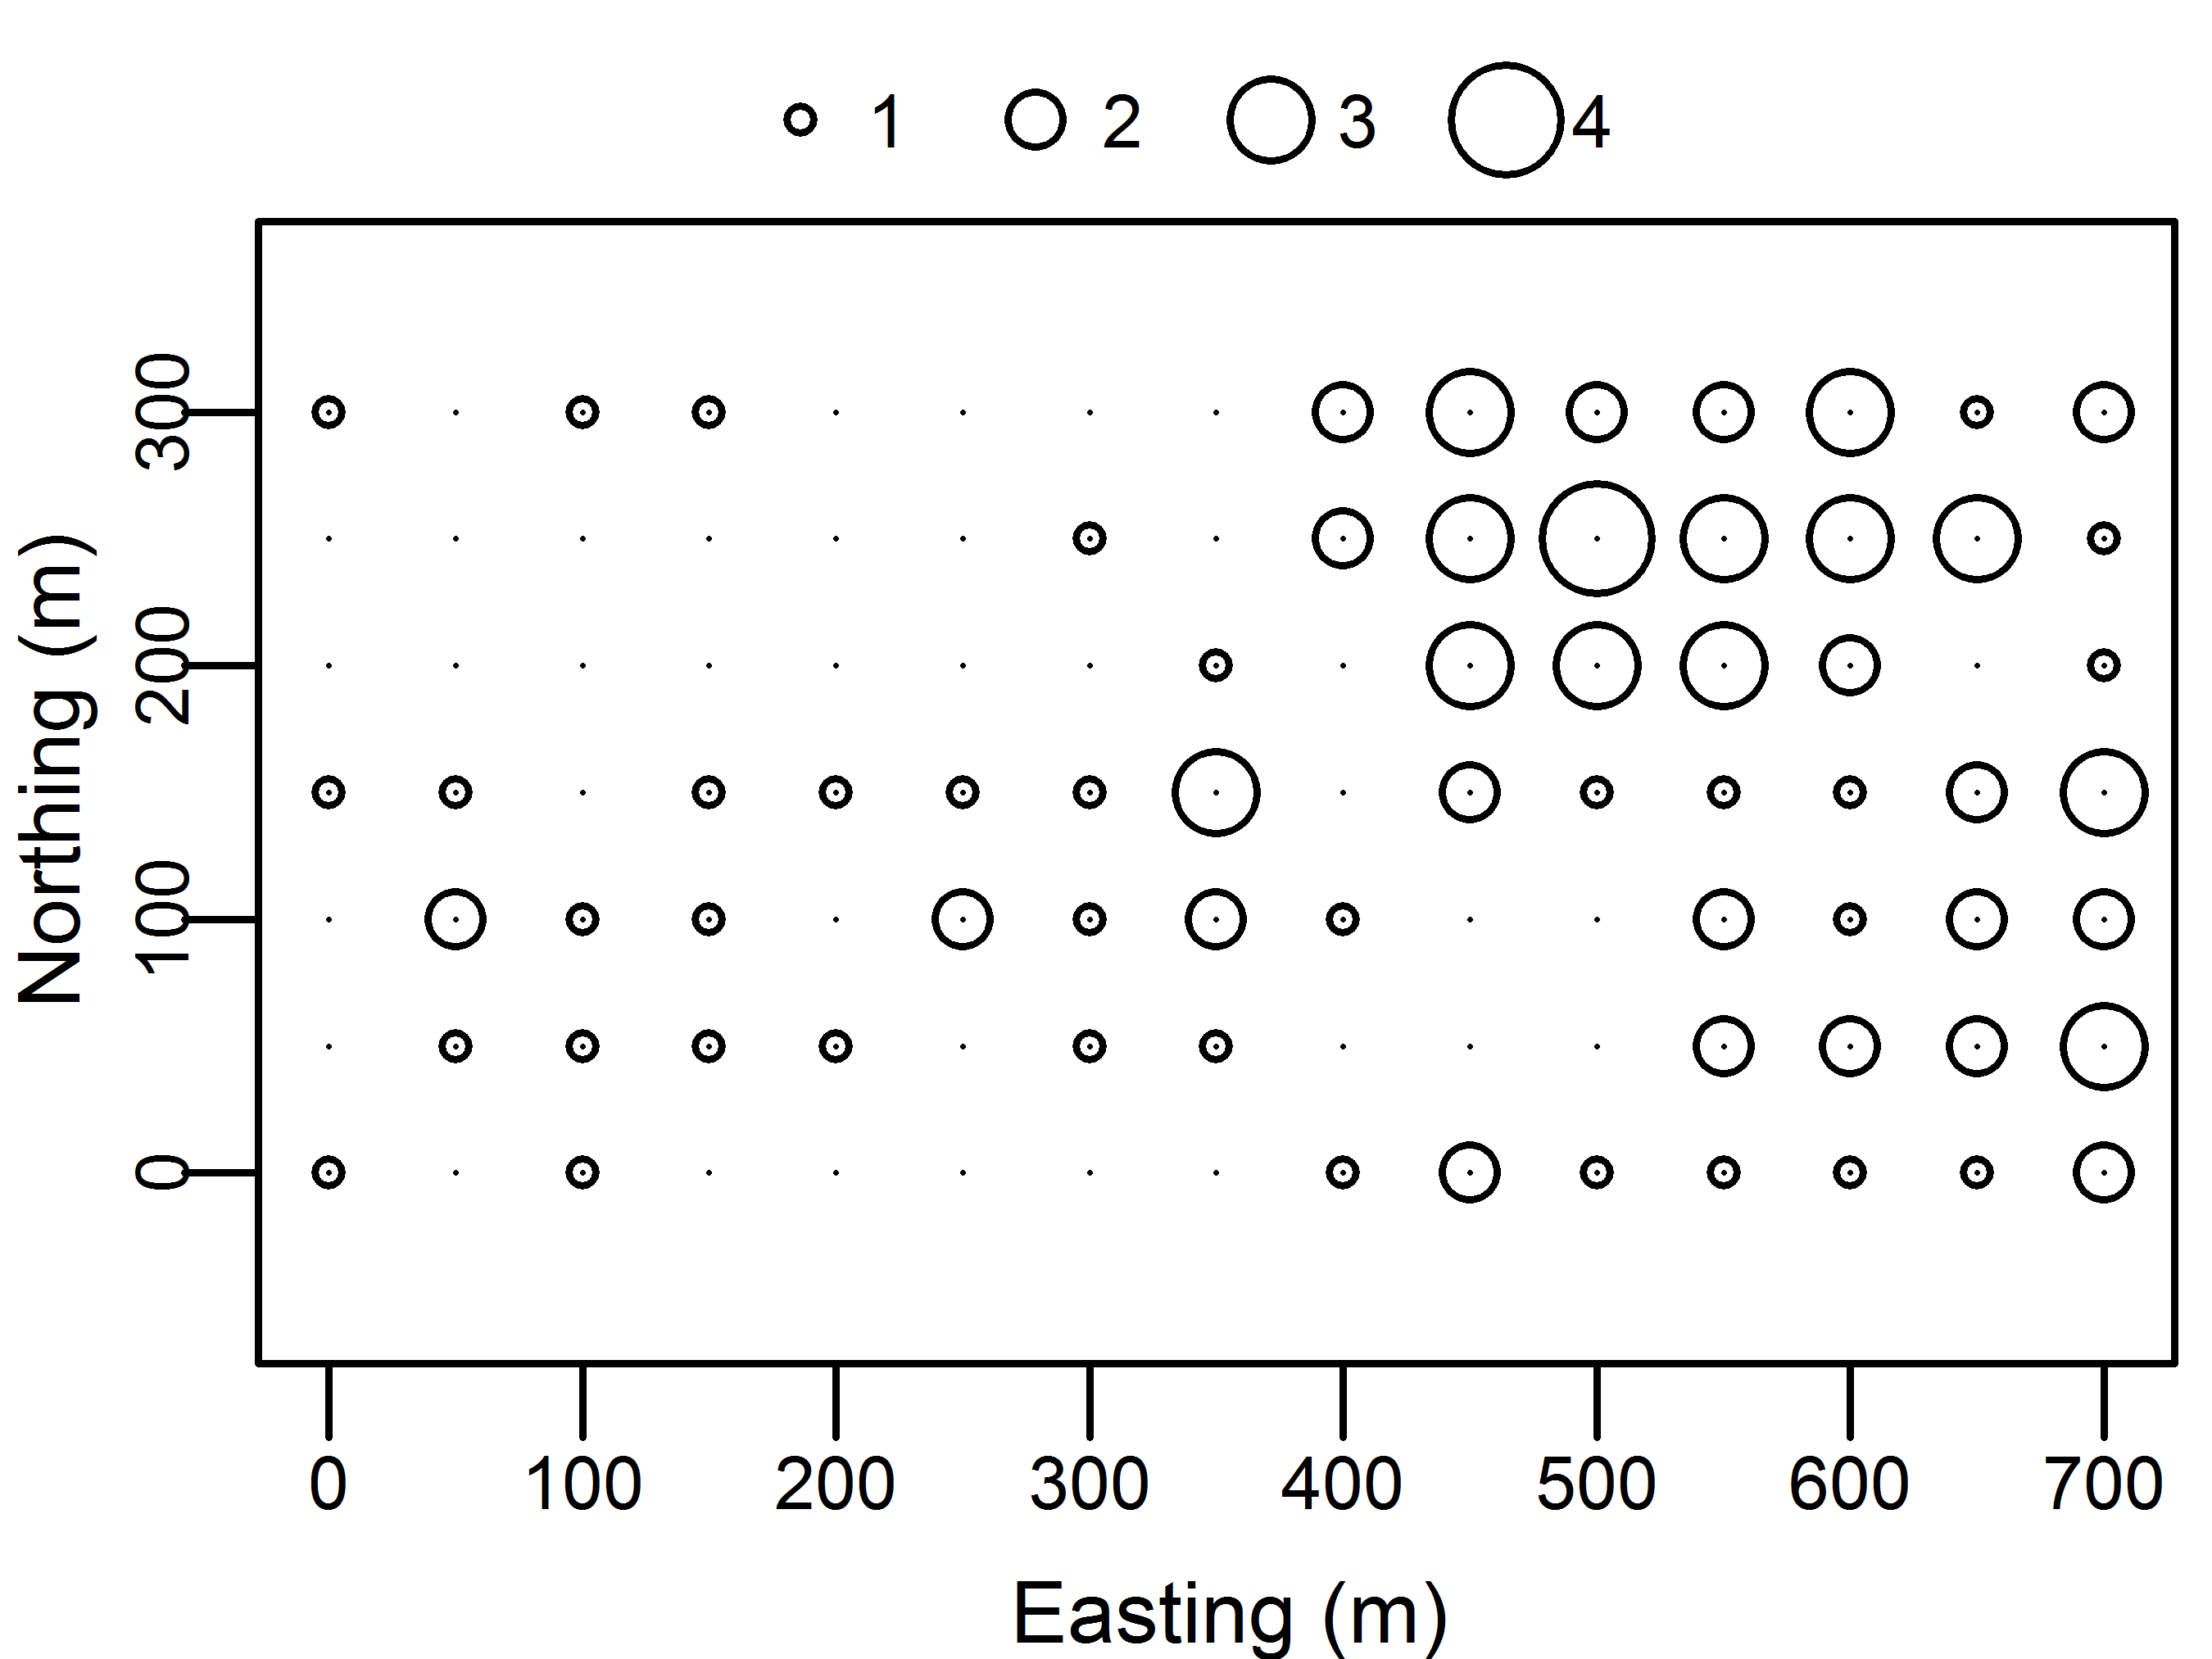
\includegraphics[width=3in,height=2.25in]{nopa.eps}
  \caption{Spatially-correlated counts of northern parula on a 50-m
    grid. The size of the circle represents the total number of
    detections at each point.}
  \label{fig:nopaDat}
\end{figure}

%\end{comment}


In our analysis of the parula data, we defined the point process
state-space by buffering the grid of point
count locations by 250 m and used $M=300$. We simulated posterior
distributions using three Markov chains,
each consisting of 300000 iterations after discarding the initial 10000
draws. Convergence was satisfactory, as indicated by an $\hat{R}$
statistic of $<$ 1.02 \citep{gelmanRubin92}.

One benefit of a Bayesian analysis is that it can accommodate prior
information on the home range size and encounter rate parameters,
which are readily available for many
species. To illustrate, we analyzed the parula data using two sets of
priors. In the first set, all priors were
improper, customary non-informative priors (see Table \ref{t:nopaPosts}).
Uniform priors were also used in the second set, with the exception of
an informative prior for the scale parameter $\sigma \sim
\mbox{Gamma}(13,10)$. We arrived at this prior using the methods
described by \citet{royleEA11_search} and published
information on the warbler's home range size and detection probability
\citep{Moldenhaer_NOPAbna,SimonsEA09}. More details on this
derivation are found in \ref{suppA}. We briefly note here that this prior
includes the biologically-plausible range of values from $\sigma$
suggested by the published literature.

The posterior distribution for
$N$ was highly skewed with a long right tail resulting in a wide 95\%
credible interval (Table \ref{t:nopaPosts}). Nonetheless, the interval
for density, $D$, includes estimates reported from more intensive field
studies \citep[][]{Moldenhaer_NOPAbna}. This was true when considering
both sets of priors, although posterior precision was higher under the
informative set of priors. Specifically, the use of prior information
reduced posterior density at high, biologically implausible,
values of $\sigma$, and hence decreased the posterior mass for
low values of $N$ (Fig.~\ref{fig:prior}).

In addition to estimating density, our model can be used to produce
density surface maps, which are often used in applied ecological
research to direct management efforts and develop hypotheses regarding
the factors influencing abundance.
Density surface maps can be produced by discretized the
state-space and tallying the number of activity centers occurring in
each pixel during each MCMC iteration. Parula density was
highest near the northeastern corner of the study plot, which may
correspond to important habitat features such as suitable nest site
locations (Fig.~\ref{fig:nopaDen}). We anticipate future model
extensions to directly model the
point process intensity using habitat covariates.


\begin{table}%[t]
  \caption{Posterior summary statistics for spatial Poisson-count
    model applied to the northern parula data. Two sets of priors were
    considered. $M=300$ was used in both cases. Parulas/ha, $D$, is a
    derived parameter.}
  \scriptsize
  \begin{tabular}{l l rrrrrr}
    \hline
    Par        & Prior                  & Mean  & SD    & Mode   & q0.025  & q0.50  & q0.975  \\
    \hline
    $\sigma$   & $U(0, \infty)$   & 2.154   & 1.222  & 1.230   & 0.896   & 1.665   & 5.170    \\
    $\lambda_0$ & $U(0, \infty)$  & 0.284   & 0.149 & 0.212    & 0.084  & 0.256  & 0.665   \\
    $N$        & $U(0, M)$             & 40.953   & 38.072  & 4.000  & 3.000       & 31.000     & 143.000     \\
    $D$        &  --                   & 0.427    & 0.397 & 0.0417   & 0.0313  & 0.323  & 1.490    \\
    \hline
    $\sigma$    & $G(13, 10)$          & 1.301    & 0.258 & 1.230    & 0.889   & 1.266   & 1.908    \\
    $\lambda_0$ & $U(0, \infty)$ & 0.298    & 0.132 & 0.240    & 0.098   & 0.279  & 0.603   \\
    $N$         & $U(0, M)$            & 59.321   & 36.489  & 36.000 & 18.000      & 50.000     & 157.000     \\
    $D$         &  --                  & 0.618    & 0.380 & 0.375   & 0.188   & 0.521  & 1.635    \\
    \hline
  \end{tabular}
  \label{t:nopaPosts}
\vspace{0.5cm}
\end{table}


%\begin{comment}

\begin{figure}
  \centering
  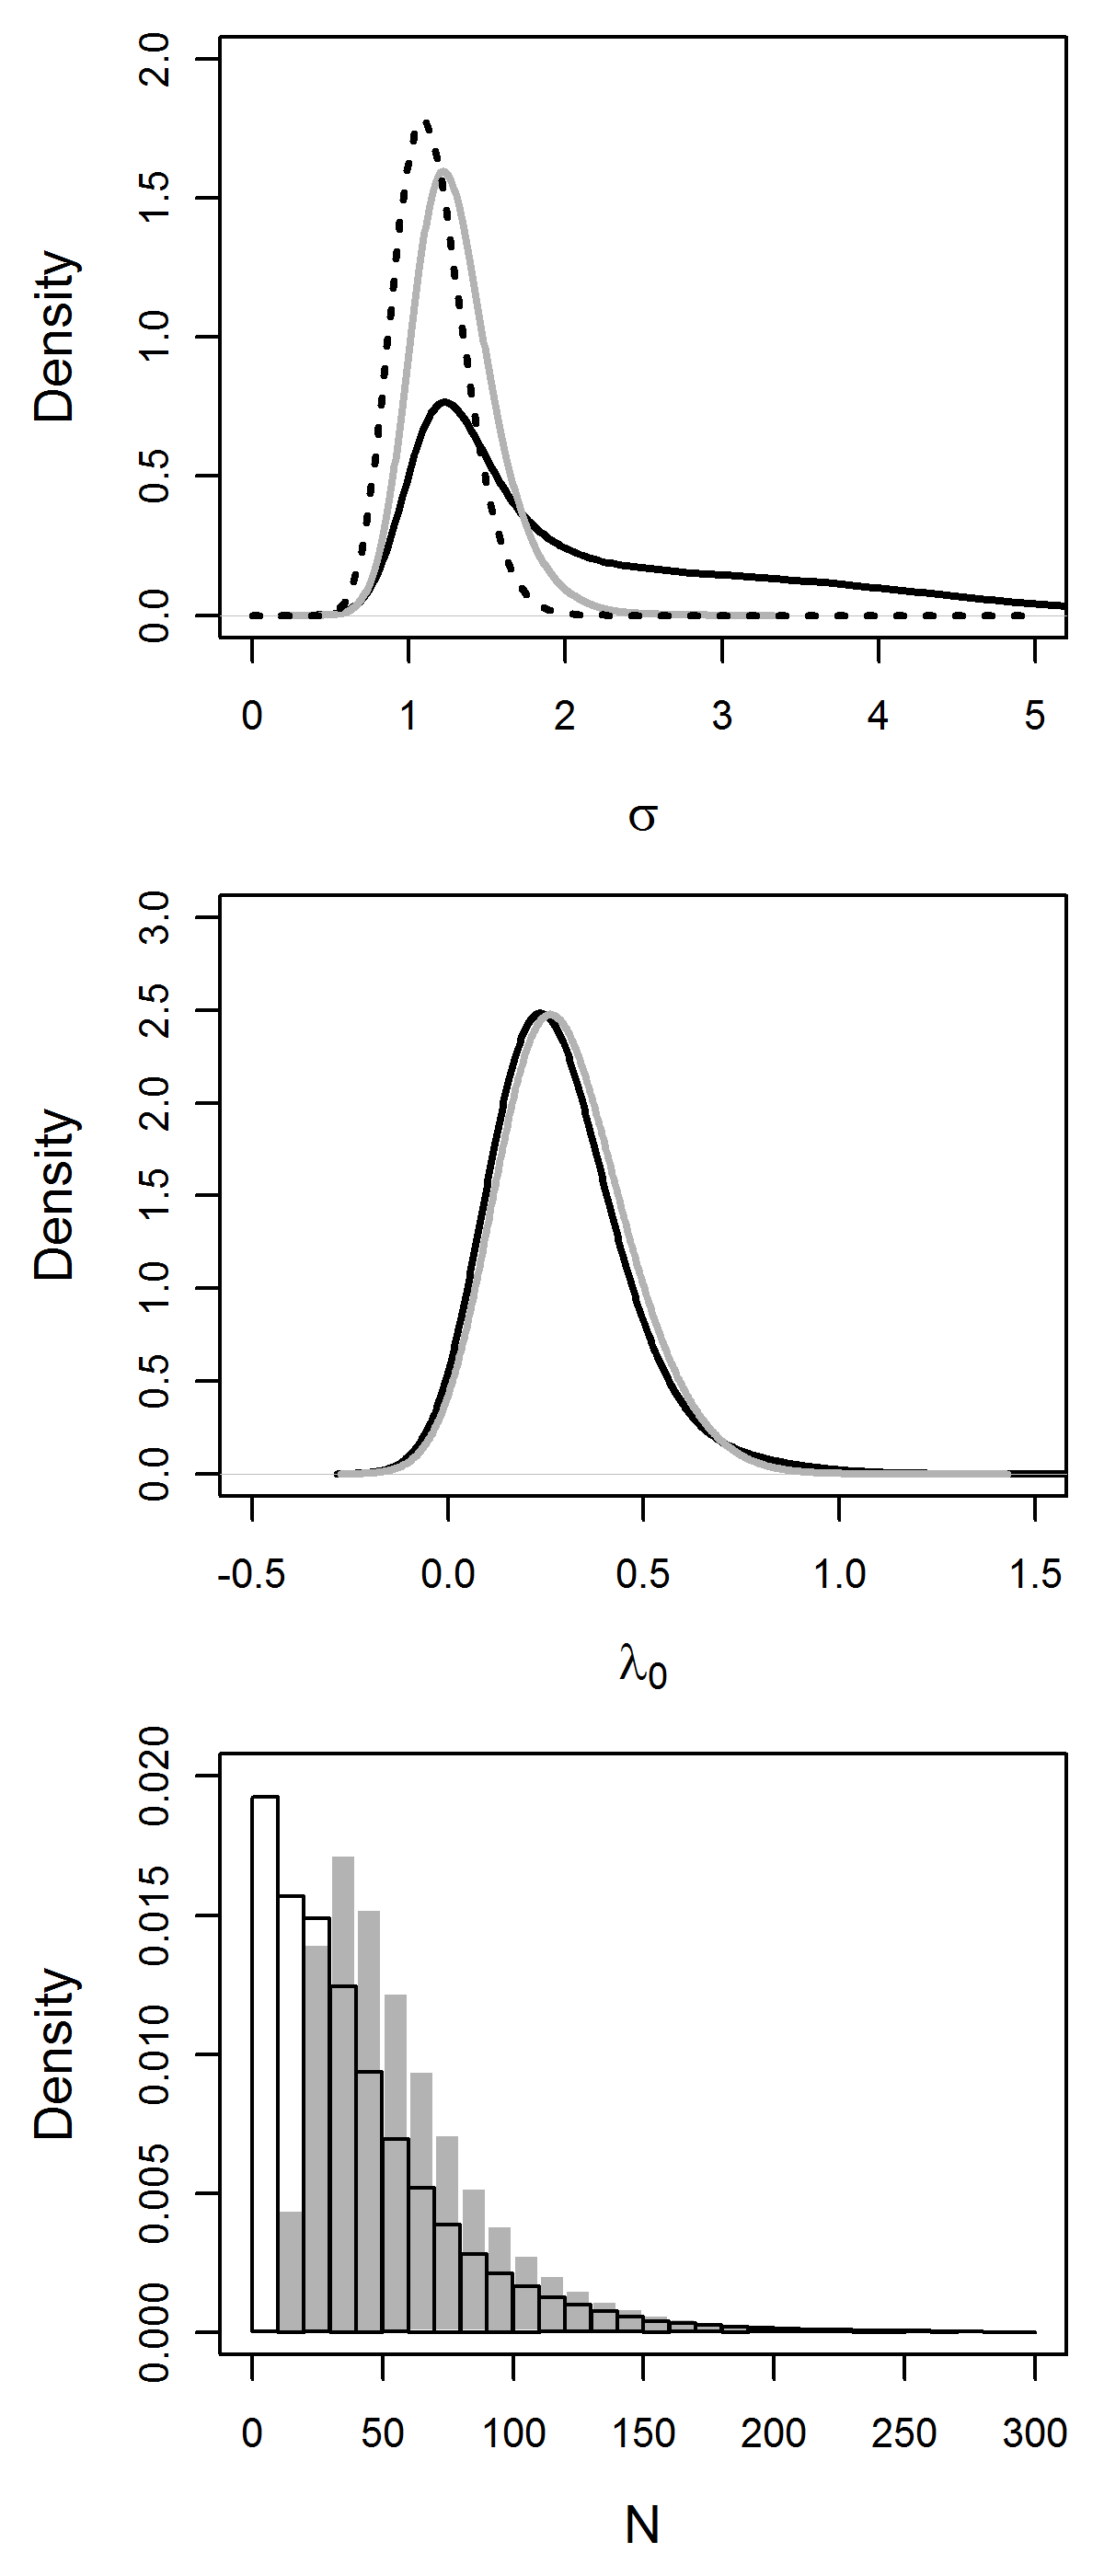
\includegraphics[width=1.5in,height=3in]{prior.eps} % was 3,7
  \caption{Effects of $\sigma \sim \mbox{Gamma}(13,10)$
    prior on the posterior distributions from the northern parula
    model. Posteriors from model with uniform priors are
    shown in black, and posteriors from the informative prior model
    are shown in gray. The prior itself is shown as dotted line in the
    upper panel.}
  \label{fig:prior}
\end{figure}




\begin{figure}
  \centering
  \includegraphics[width=3in,height=2.25in]{nopaDen2.eps}
  \caption{Estimated density surface of northern parula activity
    centers. The grid of point count locations with count totals is
    superimposed. See Fig. 1 for additional details.  }
  \label{fig:nopaDen}
\end{figure}

%\end{comment}



\section{On (Im)precision}





\section{How Much Correlation Is Enough?}



\section{Mutants}

\subsection{Other observation models}

\subsection{Linear designs}




\section{Summary}








In this paper, we confronted one of the most difficult challenges
faced in wildlife sampling ---
estimation of density in the absence of data to distinguish among
individuals. To do so, we developed a novel class of
spatially-explicit models that
applies to spatially organized counts, where the count locations or
devices are located sufficiently close together so that individuals
are exposed to encounter at multiple devices. This design yields
correlation in the observed counts, and this correlation proves to be
informative about encounter probability parameters and hence density.
We note that sample locations in count-based studies are typically
{\it not} organized close
together in space because conventional wisdom and standard practice
dictate that independence of sample units is necessary
\citep{hurlbert84_pseudorep}. Our model
suggests that in some cases it might be advantageous to deviate from
the conventional wisdom if one is interested in direct inference about
density. Of course, this is also known in the application of standard spatial
capture-recapture  models \citep{borchersEfford08_scr}
where individual
identity is preserved across trap encounters, but it is seldom, if
ever, considered in the design of more traditional count surveys.

Our model has broad relevance to an incredible number of animal
sampling problems. Our motivating problem involved bird point counts
where individual
identity is typically not available. The model also applies
to other standard methods used to sample unmarked
populations,  such as camera traps
or even methods that yield sign ({\it e.g.} scat, track) counts
indexed by space. However, results of our simulation study reveal some
important limitations of the basic
estimator applied to situations in which none of the individuals can
be uniquely identified. In particular, posterior
distributions are highly skewed in typical small to moderate sample
size situations and posterior precision is low.

Several modifications of the model can lead to improved
performance of the estimator.
Our simulation results demonstrate that marking a subset of
individuals can yield substantial increases in posterior
precision. Marking a subset of individuals is
commonplace is animal studies such as when a small number of individuals are
radio-collared in conjunction with a count-based survey
\citep{bartmannEA:87}. In many other situations a subset of
individuals can be identified by natural marks alone, and thus our
model could be applied to data from camera-trapping studies of
species such as mountain lions, deer, coyotes for which traditional
SCR methods are not effective \citep{kellyEA:puma:08}.
Thus, the ability to study partially-marked populations
adds flexibility to existing SCR methods, and also
creates new opportunities for designing efficient SCR studies
since the costs of marking all individuals in a population can be
prohibitive.

We note the existence of traditional approaches to combining data on
marked and unmarked animals based on either the Lincoln-Peterson
estimator or so-called ``mark-resight'' methods.
\citep{bartmannEA:87, mintaMangel:89, mcclintockHoeting:09}. In their
simplest form, mark-resight methods involve fitting standard
closed-population mark-recapture models to the data on marked
individuals, and the resultant estimate of detection probability
($\hat{p}$) is used to estimate population size as $\hat{N} = m +
u/\hat{p}$ where $m$ and $u$ are the number of
marked and unmarked individual, respectively. In this case,
the unmarked individuals provide no information about the
encounter rate parameters, and thus mark-resight methods cannot be
used unless a large sample of marked individuals is available. This
contrasts with our approach which can be used even when all
individuals are unmarked.

In some cases, such as in point counts of birds, it may not be
practical to mark individuals. An alternative to increasing posterior
precision is to utilize prior information on
home range size. Indeed, extensive information on home range size has
been compiled for many species in diverse habitats %\emph{e.g.}
\citep[\emph{e.g.},][]{degraafYamasaki:01}. It is
easy to embody this information in a prior distribution as we
demonstrated for the parula data.

An additional design extension that could increase precision is to use
multiple sampling methods, in which one method generates encounter
frequencies and the other method generates individuality.
For example, camera traps are now commonly used with surveys for
sign (scat or tracks), or hair snares for sampling bear populations.
These distinct methods would have different basal detection
rates but share an underlying spatial model describing the
organization of individuals in space.
Our models show promise for using
these disparate data types efficiently
for estimating density.


\subsection{$N$-mixture models}

Parallel developments which appear ostensibly
orthogonal to SCR models have addressed the problem of estimating
population size when individuals are unmarked. So-called
$N$-mixture models \citep{royle04a, royle04b, royle_distsamp_2004}
can be applied to a repeated-measures type of data structure
wherein  data are collected at $R$ sites, with $J$
replicate surveys are conducted at each.
$N$-mixture models regard abundance at each site ($N_r$) as an
{\it i.i.d.} realization of a discrete distribution such as the
Poisson or negative binomial with expectation $\theta$. In the
standard binomial $N$-mixture model, the observed counts are
treated as binomial outcomes with $N_r$ ``trials" and detection
probability $p$.

Although these models have proven useful for studies of factors that
affect variation in abundance, interpretation of model parameters is
strongly dependent on the assumption that populations are
closed with respect to demographic processes and movement. The closure
assumption can be an important practical limitation
\citep[but see][]{dailMadsen11, chandlerEA11_tempem}. Furthermore the
{\it i.i.d.} assumption is violated if spatial
correlation exists among sites, such as if animals move among plots.
Although we formulated the model developed in our paper as
an extension of spatially explicit capture-recapture models, it
clearly can
also be viewed as a spatially explicit extension of $N$-mixture models
where the local population sizes $N_{r}$ are dependent owing to the
nature of the sampling design.

Thus, two recently developed methodological frameworks, spatial
capture-recapture and $N$-mixture models, address
different problems that arise in sampling animal populations. SCR
models address non-closure by accommodating information on
the spatial organization of individuals and
juxtaposition of individuals with traps, and $N$-mixture models address
inability to uniquely identify individuals.
Our model unifies these two modeling frameworks by
addressing both issues simultaneously.


\subsection{Alternative Observation Models}
\label{ss:ext}

Several aspects of our ``spatial $N$-mixture model'' can be modified
to accommodate
alternative sampling designs or parametric distributions.
We considered situations where an individual can be detected more than
once at a trap during a single occasion, but under some designs this
is not possible. When collecting DNA samples, for instance, an
individual can often be detected at most once during an
occasion, because multiple samples of biological material cannot be
attributed
to distinct episodes. Therefore, rather than $z_{irt} \sim Poisson(\lambda_{ir})$
we have $z_{irt} \sim Bernoulli(p_{ir})$ where, for example,  $p_{ir} = p_0
exp(-d_{ir}^2/(2\sigma^2))$, and $p_0$ is the probability of
detecting an individual whose home range is centered on trap $r$. This
Bernoulli model is a focus of ongoing investigations.

Both the Poisson and the Bernoulli models
produce count observations when aggregated over individuals to form
trap-specific totals; however, ecologists often collect so-called
``detection/non-detection'' data because it can be easier to determine
if ``at least one'' individual was present rather than enumerating all
individuals in a location. In this case, the underlying $z_{irt}$
array is the same as the above cases, but we observe $y_{rt} =
I(\sum_{i=1}^{N} z_{irt} > 0)$ where $I$ is the indicator
function. This ``Poisson-binary model'' is
a spatially explicit extension of the model of
\citet{royleNichols03} in which the underlying abundance state
is inferred from binary data. We have investigated this model to a
limited extent but do not report on those results here.


\subsection{Spatial point process models}
\label{ss:similar}

Our model has some direct linkages to existing point process
models. We note that the observation intensity function (i.e.,
corresponding to the observation
locations) is a compound Gaussian kernel similar to
that of the Thomas process
\citep[pp. 61-62]{thomas:1949, moller_waagepetersen:2003}.
Also, the Poisson-Gamma Convolution models
\citep{wolpertIck_1998} are structurally similar (see also \cite{higdon1998process}
and \cite{best2000spatial}).
 In particular, our model is such a model but
with a {\it constant} basal encounter rate $\lambda_{0}$
and {\it unknown} number and location of ``support points'', which in
our case are the animal activity centers, $\bf{s_i}$.
We can thus regard our model as a model for
{\it estimating} the location and local density of support points in
such models, which we believe could be useful in the application of
convolution models.  \citet{best2000spatial} devise an MCMC algorithm for the
Poisson-Gamma model based on data augmentation, which is
similar to the component of our algorithm for
updating the $z$ variables in
the conditional-on-$z$ formulation of the model.  We emphasize that
our model is distinct from these Poisson-Gamma models
in that the number {\it and} location of such
support points are estimated.


If individuals were perfectly observable then the resulting point
process of locations is clearly a standard Poisson or Binomial (fixed
$N$) cluster process or Neyman-Scott process.
If detection is uniform over space but
imperfect, then the basic process is unaffected by this random thinning.
Our model can therefore be viewed formally as a Poisson (or Binomial)
cluster process model but one in which the thinning is
non-uniform, governed by the encounter model which dictates that
thinning rate increases with distance from the observation points. In
addition, our inference objective is, essentially, to estimate the
number of parents in the underlying Poisson cluster
process,
where the observations are biased by an incomplete sampling apparatus
(points in space).


As a model of a thinned point process, our model has much in common
with classical distance sampling models \citep{buckland_introduction_2001}.
The main distinction is that our data structure does {\it not} include
observed distances, although the underlying observation model is
fundamentally the same as in distance sampling if there is only a
single replicate sample and $\bf{s}_i$ is defined as an individual's
location at an instant in time. For replicate samples, our model preserves
(latent) individuality across samples and traps which is not a feature
of distance sampling. We note that error in measurement of distance is
not a relevant consideration in our model, and we explicitly do not
require the standard distance sampling assumption that the probability
of detection is 1 if an individual occurs at the survey point. More
importantly, distance sampling models cannot be applied to data from
many of the sampling designs for which our model is relevant. For
example, many rare and endangered species can only be
effectively surveyed using methods such as hair snares and camera
traps that do not produce distance data \citep{oconnell10_book}.


\section{Conclusion}

Concerns about ``statistical independence'' have prompted
ecologists to design count-based studies such that observed
random variables can be regarded as {\it i.i.d.} outcomes
\citep{hurlbert84_pseudorep}. Interestingly, this
often proves impossible in practice, and elaborate
methods have been devised to model spatial dependence as a nuisance
parameter. Our paper presents a modeling framework that directly
confronts this view by demonstrating that spatial
correlation carries information about the locations of individuals,
which can be used to estimate density even when individuals
are unmarked and distance-related heterogeneity exists in encounter
probability.


